\chapter{測度論}
\label{ch:found-measure}

\subsection{可測空間と確率測度}
\label{sec:sem-measurable}

\begin{definition}{$\sigma$-代数}{sem-sigma-algebra}
  集合 $\Omega$ の部分集合族 $\mathcal{F} \subset 2^{\Omega}$（冪集合，定義~\ref{def:sem-power-set}）が
  \textbf{$\sigma$-代数}であるとは，
  以下の3条件を満たすことをいう：
  \begin{enumerate}
    \item[(i)] $\Omega \in \mathcal{F}$，
    \item[(ii)] $A \in \mathcal{F} \Longrightarrow A^c \in \mathcal{F}$（補集合で閉じる），
    \item[(iii)] $A_1, A_2, \ldots \in \mathcal{F} \Longrightarrow
      \bigcup_{k=1}^{\infty} A_k \in \mathcal{F}$（可算合併で閉じる）．
  \end{enumerate}
\end{definition}

\begin{definition}{可測空間}{sem-measurable-space}
  集合 $\Omega$ と $\Omega$ 上の定義~\ref{def:sem-sigma-algebra} $\mathcal{F}$ の組
  $(\Omega, \mathcal{F})$ を\textbf{可測空間}という．
  $\mathcal{F}$ の元を\textbf{可測集合}という．
\end{definition}

\begin{definition}{可測写像}{sem-measurable-map}
  可測空間 $(\Omega_1, \mathcal{F}_1)$ から $(\Omega_2, \mathcal{F}_2)$ への
  写像 $T \colon \Omega_1 \to \Omega_2$ が\textbf{可測}であるとは，
  $T^{-1}(A) \in \mathcal{F}_1$ がすべての $A \in \mathcal{F}_2$ に対して成り立つことをいう．
\end{definition}

\begin{definition}{ボレル $\sigma$-代数}{sem-borel}
  位相空間 $(\Omega, \mathcal{O})$ のすべての開集合
  （定義~\ref{def:sem-topological-space}）
  を含む最小の $\sigma$-代数を
  \textbf{ボレル $\sigma$-代数}といい，$\Bb(\Omega)$ と記す．
\end{definition}

\begin{definition}{可測関数}{sem-measurable-function}
  可測空間 $(\Omega, \mathcal{F})$ から $(\R, \Bb(\R))$ への可測写像
  $f \colon \Omega \to \R$（定義~\ref{def:sem-measurable-map}）を
  \textbf{可測関数}という．
  特に Polish 空間 $\X$ にボレル $\sigma$-代数 $\Bb(\X)$ を入れた
  可測空間上の可測関数を\textbf{ボレル可測関数}ともいう．
\end{definition}

\begin{definition}{積可測空間}{sem-product-measurable}
  距離空間 $(\X, d_\X)$, $(\Y, d_\Y)$ に対して，
  積空間 $\X \times \Y$ に\textbf{積距離}
  \[
    d\bigl((x, y), (x', y')\bigr) \defeq d_\X(x, x') + d_\Y(y, y')
  \]
  を入れたときのボレル $\sigma$-代数を $\Bb(\X \times \Y)$ と記し，
  可測空間 $(\X \times \Y, \Bb(\X \times \Y))$ を
  $(\X, \Bb(\X))$ と $(\Y, \Bb(\Y))$ の\textbf{積可測空間}という．
\end{definition}

\begin{definition}{射影}{sem-projection}
  距離空間 $\X$, $\Y$ の積空間 $\X \times \Y$
  （定義~\ref{def:sem-product-measurable}）に対して，
  \textbf{射影} $P_\X \colon \X \times \Y \to \X$，
  $P_\Y \colon \X \times \Y \to \Y$ を
  \[
    P_\X(x, y) \defeq x,
    \qquad
    P_\Y(x, y) \defeq y
  \]
  で定める．$P_\X$，$P_\Y$ はともに連続であり，可測写像
  （定義~\ref{def:sem-measurable-map}）でもある．
\end{definition}

\begin{definition}{測度}{sem-measure}
  可測空間 $(\Omega, \mathcal{F})$ 上の\textbf{測度}とは，
  関数 $\mu \colon \mathcal{F} \to [0, \infty]$ であって，
  次の 2 条件を満たすものをいう：
  \begin{enumerate}
    \item[(i)] $\mu(\emptyset) = 0$，
    \item[(ii)] 互いに素な可測集合 $A_1, A_2, \ldots \in \mathcal{F}$ に対して
      $\mu\bigl(\bigcup_{k=1}^{\infty} A_k\bigr) = \sum_{k=1}^{\infty} \mu(A_k)$
      （可算加法性）．
  \end{enumerate}
\end{definition}

\begin{definition}{確率測度}{sem-probability-measure}
  可測空間（定義~\ref{def:sem-measurable-space}）$(\Omega, \mathcal{F})$ 上の
  測度（定義~\ref{def:sem-measure}）$\mu$ が $\mu(\Omega) = 1$ を満たすとき，
  $\mu$ を\textbf{確率測度}という．
  $\Omega$ 上の確率測度の全体を $\Mm_+^1(\Omega)$ と記す．
\end{definition}

\subsection{測度に対する積分}
\label{sec:sem-integration}

\begin{definition}{指示関数}{sem-indicator}
  集合 $\Omega$ の部分集合 $A \subset \Omega$ に対して，
  \textbf{指示関数} $\mathbf{1}_A \colon \Omega \to \{0, 1\}$ を
  \[
    \mathbf{1}_A(y) \defeq
    \begin{cases}
      1 & y \in A, \\
      0 & y \notin A
    \end{cases}
  \]
  で定める．
\end{definition}

\begin{definition}{単関数}{sem-simple-function}
  可測空間 $(\Omega, \mathcal{F})$ 上の関数 $s \colon \Omega \to \Rnn$ が
  \textbf{単関数}であるとは，互いに素な可測集合
  $A_1, \ldots, A_m \in \mathcal{F}$ と非負定数 $c_1, \ldots, c_m \geq 0$ を用いて
  \[
    s = \sum_{k=1}^{m} c_k \mathbf{1}_{A_k}
  \]
  と表せることをいう．ここで $\mathbf{1}_{A_k}$ は
  指示関数（定義~\ref{def:sem-indicator}）である．
\end{definition}

\begin{definition}{非負可測関数の積分}{sem-nonneg-integral}
  可測空間 $(\Omega, \mathcal{F})$ 上の測度 $\mu$ に対し，
  非負可測関数の積分を以下の 2 段階で定める：
  \begin{itemize}
    \item[(i)] 単関数 $s = \sum_{k=1}^{m} c_k \mathbf{1}_{A_k}$
      （定義~\ref{def:sem-simple-function}）の積分を
      \[
        \int_\Omega s \, \d\mu \defeq \sum_{k=1}^{m} c_k \, \mu(A_k)
      \]
      で定める．
    \item[(ii)] 非負可測関数 $f \colon \Omega \to [0, \infty]$ の積分を
      \[
        \int_\Omega f \, \d\mu \defeq
        \sup\!\left\{ \int_\Omega s \, \d\mu
        \;\middle|\; s \text{ は単関数}, \; 0 \leq s \leq f \right\}
      \]
      で定める．この値は常に $[0, +\infty]$ に存在し well-defined である．
  \end{itemize}
\end{definition}

\begin{proposition}{単調収束定理と単関数近似}{sem-mct}
  可測空間 $(\Omega, \mathcal{F})$ 上の測度 $\mu$ に対して次が成り立つ．
  \begin{enumerate}
    \item[(i)] \textbf{単関数近似}：任意の非負可測関数
      $f \colon \Omega \to [0, \infty]$ に対して，
      各点で $f_n \uparrow f$ を満たす単関数の単調増加列 $(f_n)_{n \geq 1}$ が存在する．
    \item[(ii)] \textbf{単調収束定理}：
      非負可測関数の単調増加列 $f_n \uparrow f$ に対して
      $\int f_n \, \d\mu \uparrow \int f \, \d\mu$．
  \end{enumerate}
\end{proposition}

\begin{definition}{各点収束}{sem-pointwise-convergence}
  可測空間 $(\Omega, \mathcal{F})$ 上の関数列 $(f_n)_{n \geq 1}$ と
  関数 $f$ に対し，$(f_n)$ が $f$ に\textbf{各点収束}するとは，
  すべての $x \in \Omega$ で $f_n(x) \to f(x)$（$n \to \infty$）となることをいう．
\end{definition}

\begin{theorem}{有界収束定理}{sem-bounded-convergence}
  $(\Omega, \mathcal{F})$ を可測空間，$\mu$ を有限測度
  （$\mu(\Omega) < \infty$）とする．
  可測関数列 $(f_n)_{n \geq 1}$ が可測関数 $f$ に各点収束
  （定義~\ref{def:sem-pointwise-convergence}）し，
  かつある定数 $M > 0$ が存在してすべての $n$ と $x$ について
  $|f_n(x)| \leq M$ をみたすならば，
  \[
    \lim_{n \to \infty} \int_\Omega f_n \, \d\mu
    = \int_\Omega f \, \d\mu.
  \]
\end{theorem}

\begin{proof}
  \[
    g_n(x) \defeq \sup_{k \geq n} |f_k(x) - f(x)|
  \]
  とおく．$g_n$ は非負可測であり，$|f_n - f| \leq g_n$ をみたす．
  また $g_n$ は単調減少（$g_1 \geq g_2 \geq \cdots$）であり，
  $f_n \to f$ の各点収束から $g_n(x) \to 0$（すべての $x$）である．
  さらに $|f_k| \leq M$ と $|f| \leq M$ より $g_n \leq 2M$ である．

  $h_n \defeq 2M - g_n$ とおくと，$h_n$ は非負かつ単調増加で
  $h_n \uparrow 2M$ である．
  単調収束定理（命題~\ref{prop:sem-mct}）より
  \[
    \int_\Omega h_n \, \d\mu
    \;\uparrow\;
    \int_\Omega 2M \, \d\mu
    = 2M \, \mu(\Omega).
  \]
  $\mu(\Omega) < \infty$ だから
  \[
    \int_\Omega g_n \, \d\mu
    = 2M \, \mu(\Omega) - \int_\Omega h_n \, \d\mu
    \;\to\; 0.
  \]
  $|f_n - f| \leq g_n$ より
  \[
    \left|\int_\Omega f_n \, \d\mu - \int_\Omega f \, \d\mu\right|
    \leq \int_\Omega |f_n - f| \, \d\mu
    \leq \int_\Omega g_n \, \d\mu
    \to 0.  \qedhere
  \]
\end{proof}

\begin{proposition}{積分の測度に関する線形性}{sem-measure-linearity}
  可測空間 $(\Omega, \mathcal{F})$ 上の測度 $\mu_1, \ldots, \mu_n$，
  非負係数 $a_1, \ldots, a_n \geq 0$，および非負可測関数
  $f \colon \Omega \to [0, \infty]$ に対して，
  \[
    \int_\Omega f \, \d\!\Bigl(\sum_{i=1}^{n} a_i \mu_i\Bigr)
    = \sum_{i=1}^{n} a_i \int_\Omega f \, \d\mu_i.
  \]
  ここで測度の和・スカラー倍は可測集合 $A \in \mathcal{F}$ に対して
  $(\mu_1 + \mu_2)(A) \defeq \mu_1(A) + \mu_2(A)$，
  $(a\mu)(A) \defeq a\, \mu(A)$ で定まる測度である．
\end{proposition}

\begin{proof}
  単関数 $s = \sum_{k} c_k \mathbf{1}_{A_k}$ について，
  単関数積分の定義と測度の和・スカラー倍の定義から
  \[
    \int s \, \d\!\Bigl(\sum_i a_i \mu_i\Bigr)
    = \sum_k c_k \Bigl(\sum_i a_i \mu_i\Bigr)(A_k)
    = \sum_k c_k \sum_i a_i \mu_i(A_k)
    = \sum_i a_i \sum_k c_k \mu_i(A_k)
    = \sum_i a_i \int s \, \d\mu_i.
  \]
  一般の非負可測関数 $f$ に対しては，
  命題~\ref{prop:sem-mct} により単関数の単調増加列 $f_n \uparrow f$ が取れ，
  単調収束定理を両辺に適用すれば結論が得られる．
\end{proof}

\subsection{Dirac 測度と押し出し}
\label{sec:sem-dirac-pushforward}

\begin{definition}{Dirac 測度}{sem-dirac}
  可測空間 $(\Omega, \mathcal{F})$ 上の点 $x \in \Omega$ に対して，
  \textbf{Dirac 測度} $\delta_x \in \Mm_+^1(\Omega)$ を
  \[
    \delta_x(A) \defeq
    \begin{cases}
      1 & x \in A, \\
      0 & x \notin A
    \end{cases}
    \qquad (\forall\, A \in \mathcal{F})
  \]
  で定義する．すなわち指示関数（定義~\ref{def:sem-indicator}）を用いて
  $\delta_x(A) = \mathbf{1}_A(x)$ とも書ける．
\end{definition}

\begin{claim}{Dirac 測度に対する積分}{sem-dirac-integral}
  任意の非負可測関数 $f \colon \X \to [0, \infty]$ に対して，
  \[
    \int_\X f \, \d\delta_x = f(x).
  \]
\end{claim}

\begin{proof}
  $A \in \Bb(\X)$ に対し単関数積分の定義より
  $\int \mathbf{1}_A \, \d\delta_x = \delta_x(A) = \mathbf{1}_A(x)$．
  単関数 $f = \sum_k c_k \mathbf{1}_{A_k}$ に対しては積分の線形性から
  \[
    \int_\X f \, \d\delta_x
    = \sum_k c_k \, \delta_x(A_k)
    = \sum_k c_k \, \mathbf{1}_{A_k}(x)
    = f(x).
  \]
  一般の非負可測関数 $f$ に対しては，
  命題~\ref{prop:sem-mct} により単関数の単調増加列 $f_n \uparrow f$ が取れ，
  単調収束定理から
  \[
    \int_\X f \, \d\delta_x
    = \lim_{n \to \infty} \int_\X f_n \, \d\delta_x
    = \lim_{n \to \infty} f_n(x)
    = f(x).
  \]
\end{proof}

\begin{definition}{離散測度}{sem-discrete-measure}
  Polish 空間 $\X$ 上のボレル確率測度 $\mu \in \Mm_+^1(\X)$ が
  \textbf{離散測度}であるとは，
  ある $n \in \N$，相異なる $x_1, \ldots, x_n \in \X$，
  および $a_1, \ldots, a_n > 0$（$\sum_{i=1}^n a_i = 1$）が存在して
  \[
    \mu = \sum_{i=1}^{n} a_i\, \delta_{x_i}
  \]
  と表せることをいう．ここで $\delta_{x_i}$ は
  定義~\ref{def:sem-dirac}である．
\end{definition}

\begin{claim}{離散測度の表示の一意性}{sem-discrete-measure-uniqueness}
  離散測度（定義~\ref{def:sem-discrete-measure}）$\mu = \sum_{i=1}^{n} a_i\, \delta_{x_i}$ の表示について
  $a_i = \mu(\{x_i\})$ が成り立ち，
  $n$ および対 $\{(x_i, a_i)\}_{i=1}^{n}$ は $\mu$ から
  添字の入れ替えを除いて一意に定まる．
\end{claim}

\begin{proof}
  $x_1, \ldots, x_n$ は相異なるから
  $\delta_{x_i}(\{x_k\}) = \mathbf{1}[i = k]$．
  ゆえに
  \[
    \mu(\{x_k\}) = \sum_{i=1}^{n} a_i\, \delta_{x_i}(\{x_k\}) = a_k.
  \]
  もう一通りの表示
  $\mu = \sum_{j=1}^{m} b_j\, \delta_{y_j}$
  （相異なる $y_j \in \X$，$b_j > 0$，$\sum_j b_j = 1$）が存在したとすると，
  各 $y_j$ について $\mu(\{y_j\}) = b_j > 0$ より
  $y_j \in \{x_1, \ldots, x_n\}$．対称性から $\{y_j\} \subset \{x_i\}$ かつ
  $\{x_i\} \subset \{y_j\}$ ゆえ集合として一致．
  したがって $m = n$ かつある置換 $\sigma \in \Perm(n)$ で $y_{\sigma(i)} = x_i$，
  $b_{\sigma(i)} = a_i$．
\end{proof}

\begin{definition}{押し出し}{sem-pushforward}
  可測写像（定義~\ref{def:sem-measurable-map}）$T \colon \X \to \Y$ と
  確率測度（定義~\ref{def:sem-probability-measure}）$\mu \in \Mm_+^1(\X)$ に対して，
  $T$ による $\mu$ の\textbf{押し出し} $T\pushforward \mu \in \Mm_+^1(\Y)$ を
  \[
    (T\pushforward \mu)(A) \defeq \mu(T^{-1}(A))
    \qquad (\forall\, A \in \Bb(\Y))
  \]
  で定義する．
\end{definition}

\begin{proposition}{Dirac 測度と離散測度の押し出し}{sem-dirac-pushforward}
  可測写像 $T \colon \X \to \Y$ と
  押し出し（定義~\ref{def:sem-pushforward}）について，次が成り立つ．
  \begin{enumerate}
    \item[(i)] 任意の点 $x \in \X$ に対して
      $T\pushforward \delta_x = \delta_{T(x)}$．
    \item[(ii)] 任意の点 $x_1, \ldots, x_n \in \X$ と係数
      $a_1, \ldots, a_n \geq 0$ に対して
      \[
        T\pushforward \Bigl(\sum_{i=1}^{n} a_i\, \delta_{x_i}\Bigr)
        = \sum_{i=1}^{n} a_i\, \delta_{T(x_i)}.
      \]
  \end{enumerate}
\end{proposition}

\begin{proof}
  (i) 任意の $A \in \Bb(\Y)$ に対して，押し出しの定義より
  $(T\pushforward \delta_x)(A) = \delta_x(T^{-1}(A))$．
  $x \in T^{-1}(A) \iff T(x) \in A$ なので，
  \[
    \delta_x(T^{-1}(A)) =
    \begin{cases}
      1 & x \in T^{-1}(A), \text{ すなわち } T(x) \in A \\
      0 & x \notin T^{-1}(A), \text{ すなわち } T(x) \notin A
    \end{cases}
    \;=\; \delta_{T(x)}(A).
  \]

  (ii) 任意の $A \in \Bb(\Y)$ に対して，
  \begin{align*}
    \Bigl(T\pushforward \sum_i a_i \delta_{x_i}\Bigr)(A)
    &= \Bigl(\sum_i a_i \delta_{x_i}\Bigr)(T^{-1}(A))
      && \text{（押し出しの定義）} \\
    &= \sum_i a_i\, \delta_{x_i}(T^{-1}(A))
      && \text{（測度の和・スカラー倍）} \\
    &= \sum_i a_i\, \delta_{T(x_i)}(A)
      && \text{（(i) より）}
  \end{align*}
\end{proof}

%% --- 押し出しの直感略図 ---
\begin{center}
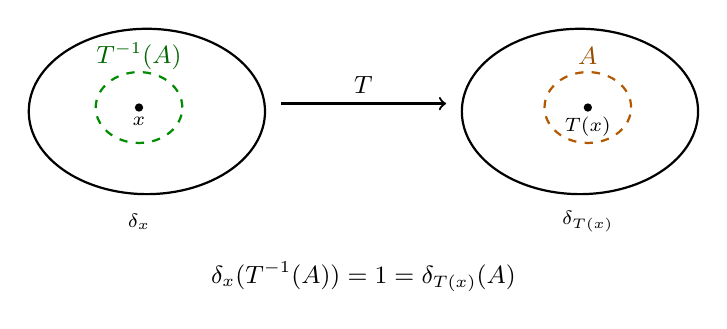
\begin{tikzpicture}[scale=1.0]
  % 左：X 側の楕円と点 x, 囲み T^{-1}(A)
  \draw[thick] (0, 0) ellipse (1.5cm and 1.05cm);
  \node[above right, font=\scriptsize, gray] at (-1.3, 0.7) {$\X$};
  \draw[dashed, thick, green!55!black]
    (-0.1, 0.05) ellipse (0.55cm and 0.45cm);
  \node[font=\small, green!40!black] at (-0.1, 0.7) {$T^{-1}(A)$};
  \fill (-0.1, 0.05) circle (1.5pt) node[below, font=\scriptsize] {$x$};

  % 矢印 T
  \draw[->, thick] (1.7, 0.1) -- (3.8, 0.1)
    node[midway, above, font=\small] {$T$};

  % 右：Y 側の楕円と点 T(x), 囲み A
  \begin{scope}[xshift=5.5cm]
    \draw[thick] (0, 0) ellipse (1.5cm and 1.05cm);
    \node[above right, font=\scriptsize, gray] at (-1.3, 0.7) {$\Y$};
    \draw[dashed, thick, orange!70!black]
      (0.1, 0.05) ellipse (0.55cm and 0.45cm);
    \node[font=\small, orange!60!black] at (0.1, 0.7) {$A$};
    \fill (0.1, 0.05) circle (1.5pt) node[below, font=\scriptsize] {$T(x)$};
  \end{scope}

  % 下：Dirac 測度の値
  \node[font=\scriptsize] at (-0.1, -1.4) {$\delta_x$};
  \node[font=\scriptsize] at (5.6, -1.4) {$\delta_{T(x)}$};
  \node[font=\small] at (2.75, -2.1)
    {$\delta_x(T^{-1}(A)) = 1 = \delta_{T(x)}(A)$};
\end{tikzpicture}
\end{center}
